\chapter{Max/MSP implementation}
\label{max}
The Max/MSP implementation is done in a modular way, so that one part of the application is analyzing sounds and the resonator is completely independent, and can be exchanged with other resonance filters(or spectral filter approaches). But even more, the resonator is it's own clipping module. It can communicate with the analysis over send/receives and stores the model it received. This way, the analysis can be run, and a resonator module can sit anywhere in another patch, being fed with the analysis. The reception of models can be turned on or off, so multiple resonator modules can be used in a modular fashion, can be fed with models individually, expose  their received models to any available pattrstorage system in their parent patcher and run on their own, not needing the analysis patch anymore, once they are set up.\\
Also, the analysis itself is kept modular, so the spectral processing, the peak finding or the audio input can easily be exchanged.
The whole structure of the Max patch follows the structure given in fig. ~\ref{fig:problem}. An overview of the complete Patch is given in fig. ~\ref{fig:maxOverview}.

\begin{figure}[H]
	\begin{center}
		\includegraphics[width = 14cm]{img/MaxOverview.png}
		\caption{An overview of the Complete Max patch}
		\label{fig:maxOverview}
	\end{center}
\end{figure}

\section{Analysis} % (fold)
    \label{sec:analysis}
 
 The analysis of the impulse response follows the steps described in figure ~\ref{fig:problem}. The impulse response is just played into a dedicated poly~ object containing several spectral processing methods. This is depicted in fig. ~\ref{fig:MaxSpectrumAnalysis}. This poly~ object is muted if no spectral processing is taking place, therefore the inefficiency of it's contents does not matter, and it can be taken advantage of a modular approach of having individual FFT and autocorrelation stages. Therefore it would be easy to add more analysis methods such as a cepstral analysis as proposed in \ref{sec:discussion}. Spectral analysis, autocorrelation, a two-pass autocorrelation and an accumulation of the autocorrelation are available here and can be compared. \\
 The peak detection in the spectral analysis can be tweaked by the user and follows the python script described in \ref{sec:python}.
The peaks that have been found are handed over to the algorithm for calculating gains and decay rates as described in \ref{sec:gainsAndDecays}.


\begin{figure}[h]
	\begin{center}
		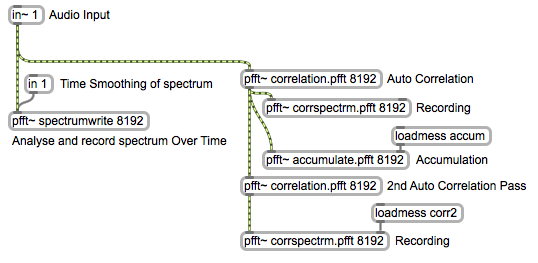
\includegraphics[width = 12cm]{img/SpectrumAnalysis.png}
		\caption{The different spectral analysis methods are performed and recorded}
		\label{fig:MaxSpectrumAnalysis}
	\end{center}
\end{figure}

In fig. \ref{fig:specwrite}, the patcher transforming the time domain signal into the frequency domain and extracting and recording magnitude data is shown. Also the vectral\~\ object performs some adjustable smoothing of the amplitude values over time. It acts similar to a low-pass filter/envelope follower on all the individual bins.  

\begin{figure}[h!]
	\begin{center}
		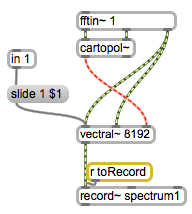
\includegraphics[width = 5cm]{SpectrumWrite.png}
		\caption{The contents of the patcher \glqq{}spectrumwrite\grqq{} }
		\label{fig:specwrite}
	\end{center}
\end{figure}



\section{Format} % (fold)
    \label{sec:format}
Temporarily, all the data is stored to three individual lists, one for the frequencies, one for the gains and one for the decay rates. These lists can be edited using a table GUI element(jit.cellblock) as shown in \ref{modelTable}.

 \begin{figure}[h]
 	\begin{center}
 		\includegraphics[width = 12cm]{img/ModelTable.png}
 		\caption{A table for viewing and editing an extracted mode model}
 		\label{modelTable}
 	\end{center}
 \end{figure}

These lists are then parsed into a format proposed by the CNMAT. This format uses text files with the following syntax:
\begin{verbatim}
ModelName1, frequency1 gain1 decayRate1 frequency2 gain2 decayRate2 (...)	decayRateN;
ModelName2, frequency1 gain1 decayRate1 frequency2 gain2 decayRate2 (...)	decayRateM;

\end{verbatim}

Storage and loading of such data is supported in this implementation.

\section{Synthesis} % (fold)
    \label{sec:synthesis}
A small synthesis section is included in the application to let the user test an analyzed model without the need of an additional Max patch. Also, this let's people, who do not own Max/MSP, design a model while hearing results, in order to save the text file and use it in other applications(such as Pure Data).  \\
Again, a modular design approach is applied. An exciter module and a resonator module were created.  \\
The exciter module incorporates two noise sources(white and pink) to choose from. These are then amplified by an AR-type envelope, which can be triggered externally. The result can be mixed with a function generator that fires an arbitrary single shot wave form, like the unit sample, \(\delta[n]\), a sinc pulse, or any user-drawn shape.
The resonator uses Max/MSP's native reson\~\ object. It loads an arbitrary number of reson\~\ objects and manages the data reception and parsing. Contained in the application is also a simple comb filter. A more detailed and realistic sound can be achieved if a setup like in fig. \ref{synth} is built for a more fine control of the sound.  

\begin{figure}[htb]
	\centering  
  	\caption{Example synthesis setup}

	\label{synth}
	\begin{tikzpicture}[auto, thick, node distance=0.5cm, >=triangle 45]
	
		\draw node at (0,0)[input] (input) {};
		
		\draw node [block, right=1.2 of input] (exciter) {\Large$Exciter$};
		\draw node [block, right= of exciter] (comb) {\Large$Comb$};
		\draw node [block, right= of comb] (EQ) {\Large$EQ$};
		\draw node [block, right= of EQ] (resonator) {\Large$Resonate$};
		\draw node [block, right= of resonator] (diff) {\Large$Diffuse$};
				
		\draw  node [output, right= of diff] (output) {};
		
		\draw[->] (input) -- node {$trigger$}(exciter);
		\draw[->] (exciter) -- node {}(comb);
		\draw[->] (comb) -- node {}(EQ);
		\draw[->] (EQ) -- node {}(resonator);
		\draw[->] (resonator) -- node {}(diff);
		\draw[->] (diff) -- node {}(output);

	\end{tikzpicture}

\end{figure}

Here, \textit{Comb} denotes a standard comb filter and \textit{Diffuse} is meant to suggest some kind of diffusion/reverberation module. For example \citep[p. 7]{schroeder_natural_1961} gives a very efficient algorithm consisting only of a couple of delays, all-passes and a feedback loop(not the commonly know Schroeder-reverb is meant here). The comb filter as well as a couple of all-passes can highly increase the perceived sound quality. An example setup for producing higher quality sound than the built-in preview resonator could look like the patch shown in fig. \ref{synthExample}. It is worth noting that both the block diagram in fig. \ref{synth} and the patch in \ref{synthExample} are actually nothing more than an accumulation of different LTI filters that are controlled in different manners. Non-linear elements are not used here, although their introduction may yield interesting results and efficiency benefits.


\begin{figure}[h]
	\begin{center}
		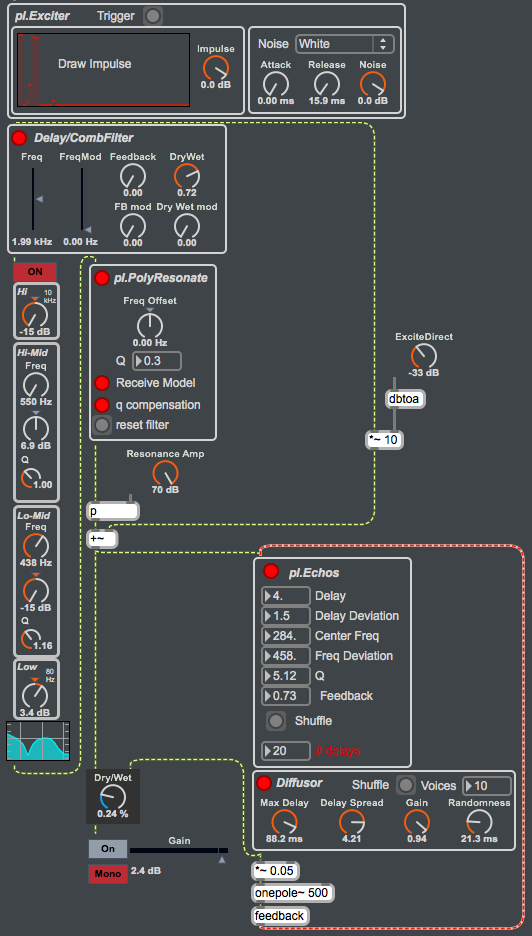
\includegraphics[width = 12cm]{img/synthExample.png}
		\caption{Example Synthesis setup}
		\label{synthExample}
	\end{center}
\end{figure}

A single resonator-patch is depicted in figure \ref{fig:reson}. Via poly\~\ this patch is instantiated multiple times, depending on how many filters are needed for a given model. Each instance calculates a \(q\) value from the given decay rate, and optionally applies a gain compensation, since rising \(q\) reduces the resulting amplitude. The \(q\) factor is calculated via an intermediate value, let's call it \(t\). The reson\~\ object's impulse response for a high \(q\) factor approaches a sinusoid, decaying by the law \(q/f=t\). Here, \(t\) is the time in which the sinusoid falls below -60 dB FS. Or one could say the filter produces \(q\) cycles of a sinusoid with frequency \(f\) before falling below -60 dB FS. This is only approximate, but good enough. This duration parameter \(t\) can easily be derived from the decay rate using the formulas given in \ref{sec:gainsAndDecays}. 

 \begin{figure}[h]
 	\begin{center}
 		\includegraphics[width = 14cm]{img/resonator.png}
 		\caption{a resonator}
 		\label{fig:reson}
 	\end{center}
 \end{figure}
 
 




